% Presentation flag: uncomment to enable presentation features (slower compilation)
\newcommand*{\PRESENTATION}

% Preliminaries
\ifdefined\PRESENTATION
	\documentclass[t]{beamer}
\else
	\documentclass[t,handout]{beamer}
\fi
\mode<presentation>
\usetheme{Warsaw}
\useoutertheme{infolines} 

% Includes
\usepackage[T1]{fontenc}
\usepackage{lmodern}
\usepackage{amsmath}
\usepackage{amsfonts}
\usepackage{bbm}
\usepackage{nicefrac}
\usepackage{color}
\usepackage{perpage}
\usepackage{tikz}
\usepackage{tikz-dependency}

\MakePerPage{footnote}

% Outline slides
\AtBeginSection
{\begin{frame} \frametitle{Outline} \tableofcontents[currentsection,currentsubsection] \end{frame}}
\AtBeginSubsection
{\begin{frame} \frametitle{Outline} \tableofcontents[currentsection,currentsubsection] \end{frame}}


\begin{document}

\title[]{Universal Semantic Parsing with Neural Networks}
\author{Daniel Hershcovich}
\institute[]{PhD Committee Meeting}
\date{October 25, 2016}

\begin{frame}
\titlepage
\end{frame}


\section{Background}

\begin{frame}
\frametitle{Semantic Annotation Schemes}
\begin{itemize}
 \item Semantic Role Labeling
 \item Semantic Dependencies
 \item Abstract Meaning Representation
 \item Universal Conceptual Cognitive Annotation
\end{itemize}
%\begin{center}
% \includegraphics[width=0.6\textwidth,keepaspectratio]{mnist}
%\end{center}
\end{frame}

\begin{frame}
\frametitle{Semantic Role Labeling (SRL)}
\centering
\vspace*{\fill}
PropBank
\vspace*{\fill}

\begin{dependency}
	\begin{deptext}[column sep=1.5em,ampersand replacement=\^]
	After \^ graduation \^ , \^ John \^ moved \^ to \^ Paris \\
	\end{deptext}
	% PropBank
	\node[xshift=4.91em,yshift=3em]{move.01}
	child{node at ($(\wordref{1}{5})$) {}};
	\node[xshift=-9.5em,yshift=3em,color=gray]{AM-TMP}
	child{node at ($(\wordref{1}{1})$) {}}
	child{node at ($(\wordref{1}{2})$) {}};
	\node[xshift=.65em,yshift=3em,color=red]{A1}
	child{node at ($(\wordref{1}{4})$) {}};
	\node[xshift=10.5em,yshift=3em,color=green]{A2}
	child{node at ($(\wordref{1}{6})$) {}}
	child{node at ($(\wordref{1}{7})$) {}};
	% FrameNet
	\node[xshift=4.91em,yshift=-3em]{Motion}
	child{node at ($(\wordref{1}{5})$) {}};
	\node[xshift=-9.5em,yshift=-3em,color=gray]{Time}
	child{node at ($(\wordref{1}{1})$) {}}
	child{node at ($(\wordref{1}{2})$) {}};
	\node[xshift=.65em,yshift=-3em,color=red]{Theme}
	child{node at ($(\wordref{1}{4})$) {}};
	\node[xshift=10.5em,yshift=-3em,color=green]{Goal}
	child{node at ($(\wordref{1}{6})$) {}}
	child{node at ($(\wordref{1}{7})$) {}};
\end{dependency}

\vspace*{\fill}
FrameNet
\end{frame}

\begin{frame}
\frametitle{Semantic Dependency Parsing (SDP)}
\centering
\vspace*{\fill}
DELPH-IN MRS-derived bi-lexical dependencies (DM)
\vspace*{\fill}

\begin{dependency}[theme=simple]
	\begin{deptext}[column sep=1.5em,ampersand replacement=\^]
	After \^ graduation \^ , \^ John \^ moved \^ to \^ Paris \\
	\end{deptext}
	\deproot{5}{top}
	\depedge{1}{2}{ARG2}
	\depedge{1}{5}{ARG1}
	\depedge{5}{4}{ARG1}
	\depedge{6}{5}{ARG1}
	\depedge{6}{7}{ARG2}
	\deproot[edge below]{5}{top}
	\depedge[edge below]{5}{2}{TWHEN}
	\depedge[edge below]{5}{4}{ACT-arg}
	\depedge[edge below]{5}{7}{DIR3-arg}
\end{dependency}

\vspace*{\fill}
Prague Dependency Treebank tectogrammatical layer (PSD)
\end{frame}

\begin{frame}
\frametitle{Abstract Meaning Representation (AMR)}
\end{frame}

\begin{frame}
\frametitle{Universal Conceptual Cognitive Annotation (UCCA)}
\centering
\vspace*{\fill}

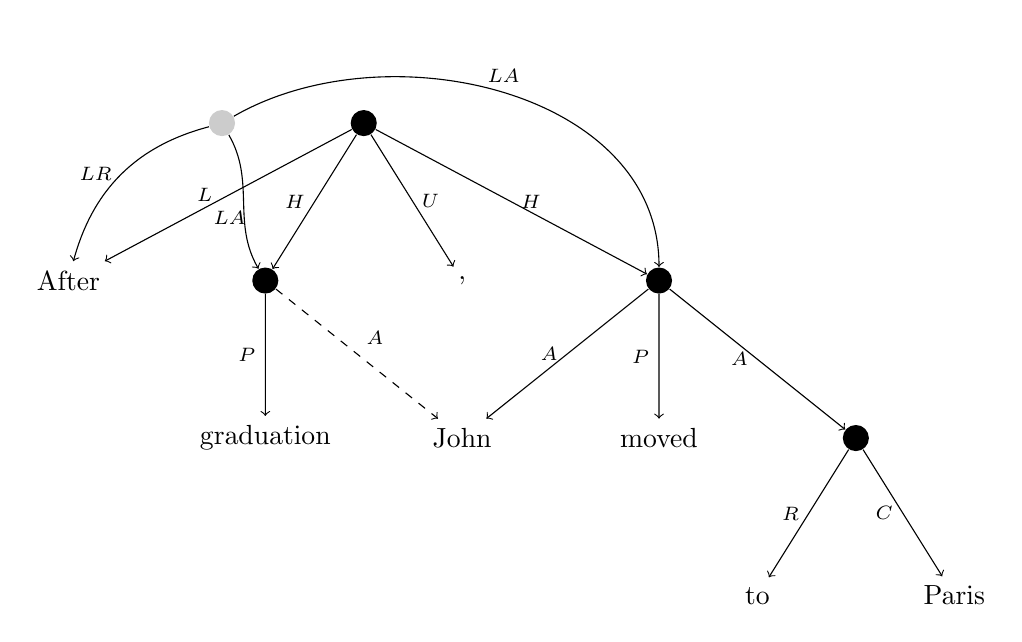
\begin{tikzpicture}[level distance=2cm, sibling distance=25mm, ->]
    \node (ROOT) [fill=black, circle] {}
      child {node (After) {After} edge from parent node[left] {\scriptsize $L$\;}}
      child {node (graduation) [fill=black, circle] {}
      {
        child {node {graduation} edge from parent node[left] {\scriptsize $P$}}
      } edge from parent node[left] {\scriptsize $H$} }
      child {node {,} edge from parent node[right] {\scriptsize $U$}}
      child {node (moved) [fill=black, circle] {}
      {
        child {node (John) {John} edge from parent node[left] {\scriptsize $A$}}
        child {node {moved} edge from parent node[left] {\scriptsize $P$}}
        child {node [fill=black, circle] {}
        {
          child {node {to} edge from parent node[left] {\scriptsize $R$}}
          child {node {Paris} edge from parent node[left] {\scriptsize $C$}}
        } edge from parent node[left] {\scriptsize $A$} }
      } edge from parent node[right] {\scriptsize $H$} }
      ;
    \draw[dashed,->] (graduation) to node [auto] {\scriptsize $A$} (John);
    \node (LKG) at (-1.8,0) [fill=black!20, circle] {};
        \draw[bend right] (LKG) to node [auto, left] {\scriptsize $LR$} (After);
        \draw (LKG) to[out=-60, in=120] node [below] {\scriptsize $LA$\quad\;} (graduation);
        \draw (LKG) to[out=30, in=90] node [above] {\scriptsize $LA$} (moved);
\end{tikzpicture}
\vspace*{\fill}
\end{frame}


\section[]{Conclusion}

\begin{frame}
\frametitle{Conclusion}
\begin{itemize}
 \item 
\end{itemize}
\end{frame}

\end{document}
